\section{Datasets and Baselines}\label{sec:simbase}

\subsection{Datasets}
\subsubsection{Simulated Datasets}
All synthetic images are generated with the image simulator of Winklmann et al.~\cite{winklmann2023}.
Fluorescence images of cesium atoms are simulated in a $3\times3$ tweezer array, with an imaging wavelength of \SI{852.3}{\nano\metre}, close to the D2 line of cesium, and a complementary metal--oxide--semiconductor (CMOS) camera model.
The complete parameter set is listed in Appendix~\ref{app:sim}. For each exposure time, one dataset is created.
There are 20 exposure times, logarithmically spaced between \SI{10}{\milli\second} and \SI{100}{\milli\second}, and every dataset contains 6002 images of $28\times28$ pixels.
The spacing is 7 pixels, which corresponds to about \SI{5}{\micro\metre} at a magnification of $6.44\times$.
This is the tightly spaced array of Phuttitarn et al.\ and Kent et al., in which the light of neighboring sites overlaps~\cite{phuttitarn2023,kent2025}.
Every site is occupied with a probability of \SI{50}{\percent} and atoms are not lost during imaging, so the label and coordinates of a site are exactly known.
The trained CNN models process a $10\times10$ pixel crop around each site, as in the CNN site of Phuttitarn et al.~\cite{phuttitarn2023}.

\subsubsection{Experimental Dataset}

The experimental dataset consists of 2024 runs of an array with 253 trap sites. Each run contains two camera images (channels) of $600\times700$ pixels.
The first channel has a higher SNR and is used to identify the sites and create the labels, whereas the second channel serves as the input to all models.
The nearest neighbors are about 26--27 pixels apart, compared with 7 pixels in the simulation, and the models process $20\times20$ pixel crops around each site instead of $10\times10$ pixel crops.
Unlike in the simulation, the occupation and site locations are unknown. The sites are identified by averaging the first channel images. The average is smoothed using a Gaussian filter ($\sigma = 2$ pixels). The resulting local maxima are the candidates, 718 in total (\cref{fig:experimental-labeling}a), and the bright component of a two-component Gaussian mixture, fitted to the heights of the candidates, retains 253 of them (\cref{fig:experimental-labeling}b).
A circular Gaussian fit within a $17\times17$ pixel window around each retained peak yields the center and the width of the site (\cref{fig:experimental-labeling}c). The score of a site in a run is the sum over all pixels of that run's first channel image, weighted by a Gaussian centered on the site with the previously fitted width of the site.
For each site, a Gaussian mixture with two components, empty and occupied, is fitted to its scores, and thus, the sites are respectively thresholded by the score at which both components are equally likely (\cref{fig:experimental-labeling}d).
On average \SI{46}{\percent} of the sites are occupied, and between \SI{34}{\percent} and \SI{52}{\percent} for individual sites. These steps use all 2024 runs and are done before the split.
The labels are therefore not the true occupation as in the simulation, but the decision on the first channel, and the fidelities on this dataset are measured against them.

\begin{figure}[H]
    \centering
    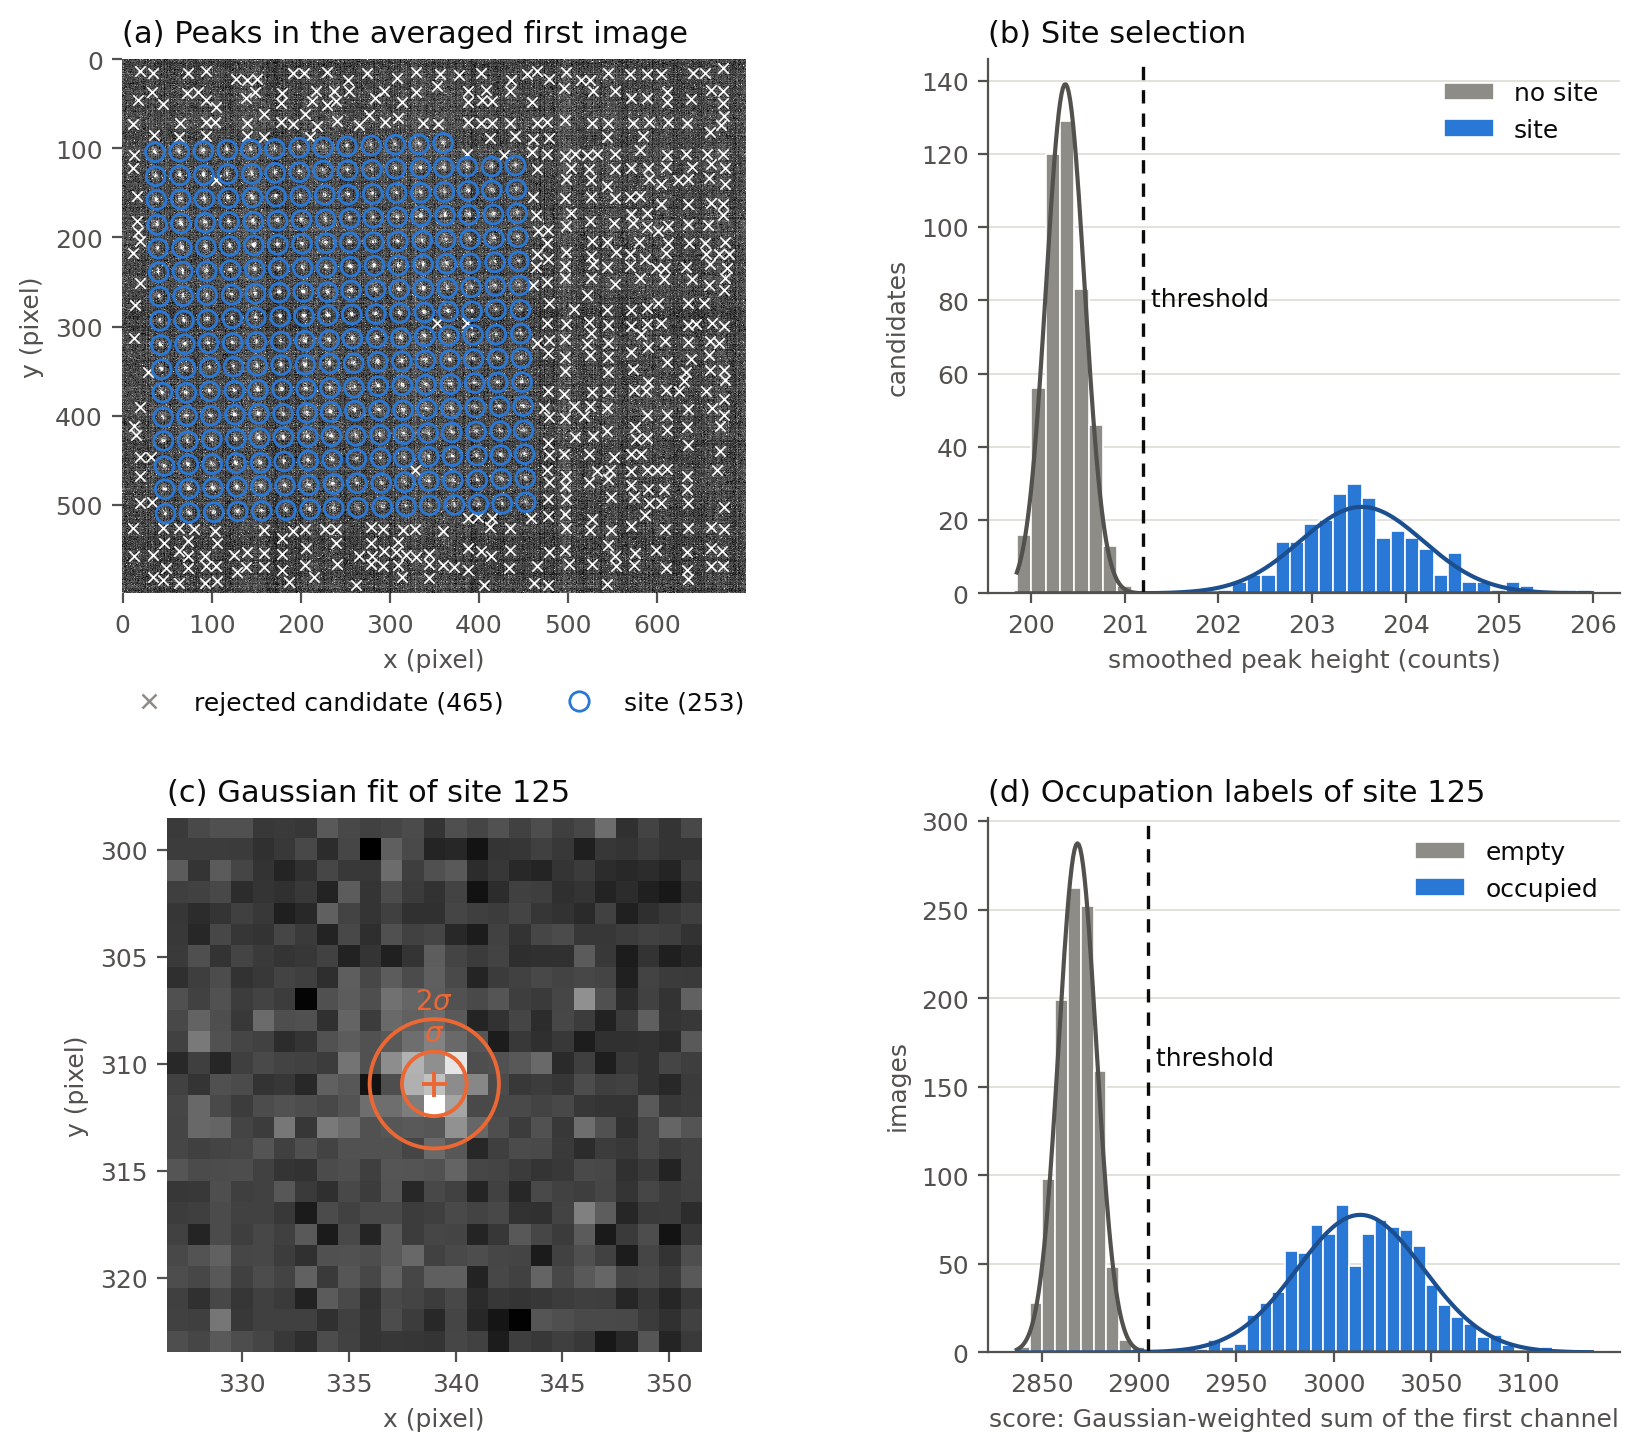
\includegraphics[width=0.95\textwidth]{experimental_labeling.png}
    \caption[Labeling workflow of the experimental dataset.]{Labeling workflow of the experimental dataset. (a) Local maxima of the smoothed average of the first channel: rejected candidates (crosses) and retained sites (circles). (b) Site selection: Peaks above the threshold are sites. (c) Circular Gaussian fit of one site (site 125) with the radii $\sigma$ and $2\sigma$. (d) Occupation labels of site 125: Scores above the threshold are labeled occupied, the others empty.}
    \label{fig:experimental-labeling}
\end{figure}


\subsubsection{Split and Normalization}

Each dataset is randomly split into \SI{60}{\percent} training, \SI{20}{\percent} validation and \SI{20}{\percent} test images, as in the experimental work~\cite{phuttitarn2023}. This results in 3601, 1200, and 1201 images for each simulated dataset, and 1214, 404, and 406 images for the experimental dataset.
The split is applied to whole images, so all sites of a given image always belong to the same subset.
Training images are used to fit the models and to compute the mean $\mu$ and the range $I_{\max}-I_{\min}$ for normalization, defined as $I' = (I-\mu)/(I_{\max}-I_{\min})$.
Validation images are used to select the checkpoint, window size, and threshold. All reported results are computed using the test images.

\subsection{Baseline Detectors}

The MF site and MF array models of Kent et al.~\cite{kent2025} and the CNN site of Phuttitarn et al.~\cite{phuttitarn2023} are used as baselines. The square and Gaussian threshold filters and the projection-based state reconstruction of Wei~\cite{wei2023}, which Winklmann et al.\ include in their comparison~\cite{winklmann2024}, serve as classical references. The matched filters are trained as in the original work: the window size $s$ is chosen on the validation images, the weights are learned by linear least squares, and the threshold is set to the value that maximizes the validation fidelity.


The CNN site has the following architecture: three $3\times3$ convolutional layers with 32, 64, and 128 filters, followed by two fully connected layers, for a total of 355\,202 trainable parameters. One model is trained per exposure time across the crops of all nine sites, using the Adam optimizer with a learning rate of $10^{-4}$, a batch size of 64, and cross-entropy loss. All hyperparameters are listed in Appendix~\ref{app:training}.


As in Kent et al.~\cite{kent2025} and Phuttitarn et al.~\cite{phuttitarn2023}, the infidelity $1-\mathcal{F}$ is defined as
\begin{equation}
 \mathcal{F} = 1 - \frac{P(B'|D) + P(D'|B)}{2},
\label{eq:fidelity}
\end{equation}
where $P(B'|D)$ is the probability that a dark site is classified as bright and $P(D'|B)$ is the probability that a bright site is classified as dark. It is evaluated on the test images for each exposure time at each site, then averaged across the nine sites.

\begin{figure}[tbp]
    \centering
    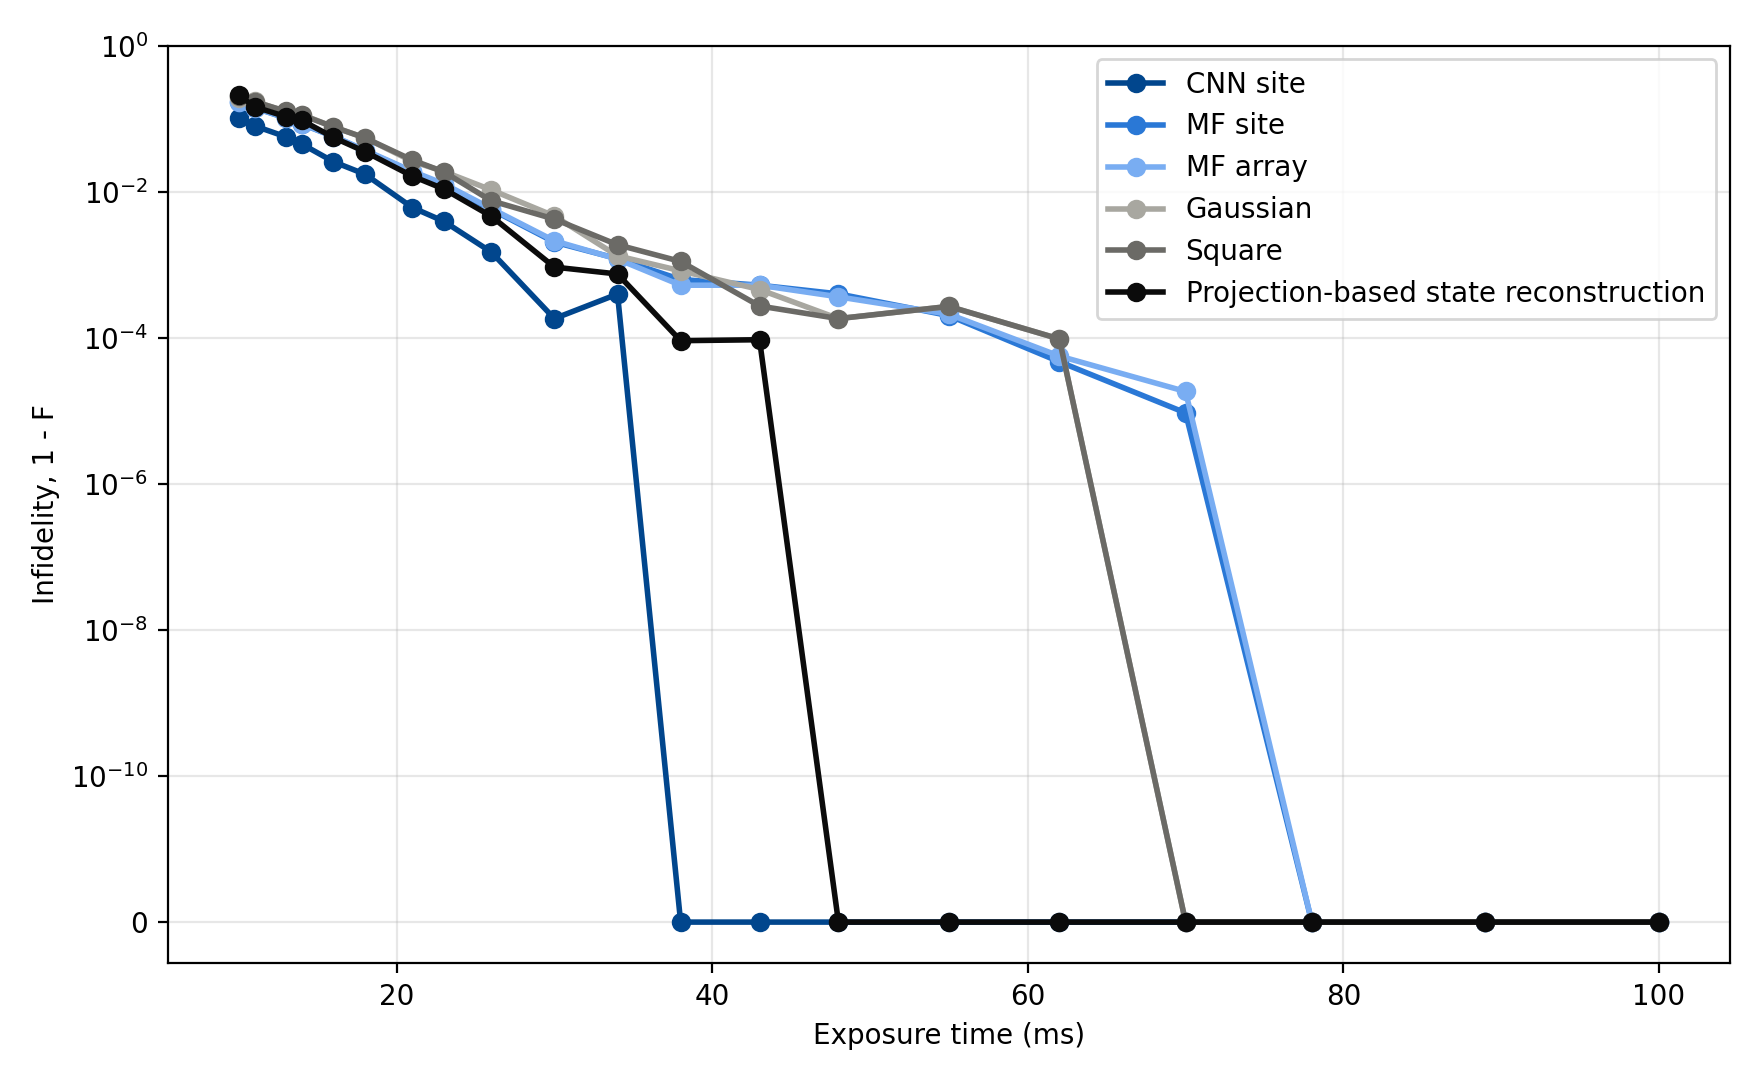
\includegraphics[width=0.85\textwidth]{fidelity_vs_exposure.png}
    \caption{Baselines infidelity versus exposure time.}
    \label{fig:baselines}
\end{figure}

\Cref{fig:baselines} shows the infidelity of all methods. It decreases with exposure time, but the CNN site is the most accurate, outperforming MF site and MF array in 17 of 20 exposure times. The remaining three are long exposures, for which both have no errors on the test set. Compared with MF site and MF array, the CNN site lowers the infidelity by about \SI{40}{\percent} at \SI{10}{\milli\second}, by about \SI{67}{\percent} at \SI{21}{\milli\second} and by about \SI{91}{\percent} at \SI{30}{\milli\second}. Its infidelity stays below $10^{-2}$ from \SI{21}{\milli\second} on, whereas the matched filters need \SI{26}{\milli\second}. The projection-based state reconstruction is the best among the other methods at medium exposures, reaching zero error at \SI{48}{\milli\second}, while the square and Gaussian filters reach zero error at \SI{70}{\milli\second}. In the experimental data of Kent et al.\ the matched filters reach about the same fidelity as the CNN site~\cite{kent2025}, whereas in the simulation, the CNN site is clearly better.

The CNN site is more accurate than the other methods, but its 355\,202 parameters and the wide convolutional layers do not allow the FPGA to meet the desired latency of a few microseconds. The next section, therefore, details how the CNN is reduced by about \SI{99}{\percent} while maintaining the same fidelity.
